\documentclass[twoside]{book}

% Packages required by doxygen
\usepackage{calc}
\usepackage{doxygen}
\usepackage{graphicx}
\usepackage[utf8]{inputenc}
\usepackage{makeidx}
\usepackage{multicol}
\usepackage{multirow}
\usepackage{textcomp}
\usepackage[table]{xcolor}

% Font selection
\usepackage[T1]{fontenc}
\usepackage{mathptmx}
\usepackage[scaled=.90]{helvet}
\usepackage{courier}
\usepackage{amssymb}
\usepackage{sectsty}
\renewcommand{\familydefault}{\sfdefault}
\allsectionsfont{%
  \fontseries{bc}\selectfont%
  \color{darkgray}%
}
\renewcommand{\DoxyLabelFont}{%
  \fontseries{bc}\selectfont%
  \color{darkgray}%
}

% Page & text layout
\usepackage{geometry}
\geometry{%
  a4paper,%
  top=2.5cm,%
  bottom=2.5cm,%
  left=2.5cm,%
  right=2.5cm%
}
\tolerance=750
\hfuzz=15pt
\hbadness=750
\setlength{\emergencystretch}{15pt}
\setlength{\parindent}{0cm}
\setlength{\parskip}{0.2cm}
\makeatletter
\renewcommand{\paragraph}{%
  \@startsection{paragraph}{4}{0ex}{-1.0ex}{1.0ex}{%
    \normalfont\normalsize\bfseries\SS@parafont%
  }%
}
\renewcommand{\subparagraph}{%
  \@startsection{subparagraph}{5}{0ex}{-1.0ex}{1.0ex}{%
    \normalfont\normalsize\bfseries\SS@subparafont%
  }%
}
\makeatother

% Headers & footers
\usepackage{fancyhdr}
\pagestyle{fancyplain}
\fancyhead[LE]{\fancyplain{}{\bfseries\thepage}}
\fancyhead[CE]{\fancyplain{}{}}
\fancyhead[RE]{\fancyplain{}{\bfseries\leftmark}}
\fancyhead[LO]{\fancyplain{}{\bfseries\rightmark}}
\fancyhead[CO]{\fancyplain{}{}}
\fancyhead[RO]{\fancyplain{}{\bfseries\thepage}}
\fancyfoot[LE]{\fancyplain{}{}}
\fancyfoot[CE]{\fancyplain{}{}}
\fancyfoot[RE]{\fancyplain{}{\bfseries\scriptsize Generated on Mon May 11 2015 19\-:23\-:21 for My Project by Doxygen }}
\fancyfoot[LO]{\fancyplain{}{\bfseries\scriptsize Generated on Mon May 11 2015 19\-:23\-:21 for My Project by Doxygen }}
\fancyfoot[CO]{\fancyplain{}{}}
\fancyfoot[RO]{\fancyplain{}{}}
\renewcommand{\footrulewidth}{0.4pt}
\renewcommand{\chaptermark}[1]{%
  \markboth{#1}{}%
}
\renewcommand{\sectionmark}[1]{%
  \markright{\thesection\ #1}%
}

% Indices & bibliography
\usepackage{natbib}
\usepackage[titles]{tocloft}
\setcounter{tocdepth}{3}
\setcounter{secnumdepth}{5}
\makeindex

% Hyperlinks (required, but should be loaded last)
\usepackage{ifpdf}
\ifpdf
  \usepackage[pdftex,pagebackref=true]{hyperref}
\else
  \usepackage[ps2pdf,pagebackref=true]{hyperref}
\fi
\hypersetup{%
  colorlinks=true,%
  linkcolor=blue,%
  citecolor=blue,%
  unicode%
}

% Custom commands
\newcommand{\clearemptydoublepage}{%
  \newpage{\pagestyle{empty}\cleardoublepage}%
}


%===== C O N T E N T S =====

\begin{document}

% Titlepage & ToC
\hypersetup{pageanchor=false}
\pagenumbering{roman}
\begin{titlepage}
\vspace*{7cm}
\begin{center}%
{\Large My Project }\\
\vspace*{1cm}
{\large Generated by Doxygen 1.8.6}\\
\vspace*{0.5cm}
{\small Mon May 11 2015 19:23:21}\\
\end{center}
\end{titlepage}
\clearemptydoublepage
\tableofcontents
\clearemptydoublepage
\pagenumbering{arabic}
\hypersetup{pageanchor=true}

%--- Begin generated contents ---
\chapter{Hierarchical Index}
\section{Class Hierarchy}
This inheritance list is sorted roughly, but not completely, alphabetically\-:\begin{DoxyCompactList}
\item \contentsline{section}{component\-Test}{\pageref{classcomponentTest}}{}
\item Serializable\begin{DoxyCompactList}
\item \contentsline{section}{Convertor}{\pageref{classConvertor}}{}
\item \contentsline{section}{Noise\-Function}{\pageref{classNoiseFunction}}{}
\item \contentsline{section}{Sample}{\pageref{classSample}}{}
\item \contentsline{section}{Sample\-Reader}{\pageref{classSampleReader}}{}
\end{DoxyCompactList}
\end{DoxyCompactList}

\chapter{Class Index}
\section{Class List}
Here are the classes, structs, unions and interfaces with brief descriptions\-:\begin{DoxyCompactList}
\item\contentsline{section}{\hyperlink{classcomponentTest}{component\-Test} }{\pageref{classcomponentTest}}{}
\item\contentsline{section}{\hyperlink{classConvertor}{Convertor} }{\pageref{classConvertor}}{}
\item\contentsline{section}{\hyperlink{classNoiseFunction}{Noise\-Function} }{\pageref{classNoiseFunction}}{}
\item\contentsline{section}{\hyperlink{classSample}{Sample} }{\pageref{classSample}}{}
\item\contentsline{section}{\hyperlink{classSampleReader}{Sample\-Reader} }{\pageref{classSampleReader}}{}
\end{DoxyCompactList}

\chapter{Class Documentation}
\hypertarget{classcomponentTest}{\section{component\-Test Class Reference}
\label{classcomponentTest}\index{component\-Test@{component\-Test}}
}
\subsection*{Static Public Member Functions}
\begin{DoxyCompactItemize}
\item 
static void \hyperlink{classcomponentTest_adab11c89a363b9704a11ed3c5f79e571}{main} (String\mbox{[}$\,$\mbox{]} args)
\end{DoxyCompactItemize}


\subsection{Detailed Description}
\begin{DoxyAuthor}{Author}
no\-\_\-author 
\end{DoxyAuthor}


\subsection{Member Function Documentation}
\hypertarget{classcomponentTest_adab11c89a363b9704a11ed3c5f79e571}{\index{component\-Test@{component\-Test}!main@{main}}
\index{main@{main}!componentTest@{component\-Test}}
\subsubsection[{main}]{\setlength{\rightskip}{0pt plus 5cm}static void component\-Test.\-main (
\begin{DoxyParamCaption}
\item[{String\mbox{[}$\,$\mbox{]}}]{args}
\end{DoxyParamCaption}
)\hspace{0.3cm}{\ttfamily [inline]}, {\ttfamily [static]}}}\label{classcomponentTest_adab11c89a363b9704a11ed3c5f79e571}

\begin{DoxyParams}{Parameters}
{\em args} & \\
\hline
\end{DoxyParams}


The documentation for this class was generated from the following file\-:\begin{DoxyCompactItemize}
\item 
component\-Test.\-java\end{DoxyCompactItemize}

\hypertarget{classConvertor}{\section{Convertor Class Reference}
\label{classConvertor}\index{Convertor@{Convertor}}
}
Inheritance diagram for Convertor\-:\begin{figure}[H]
\begin{center}
\leavevmode
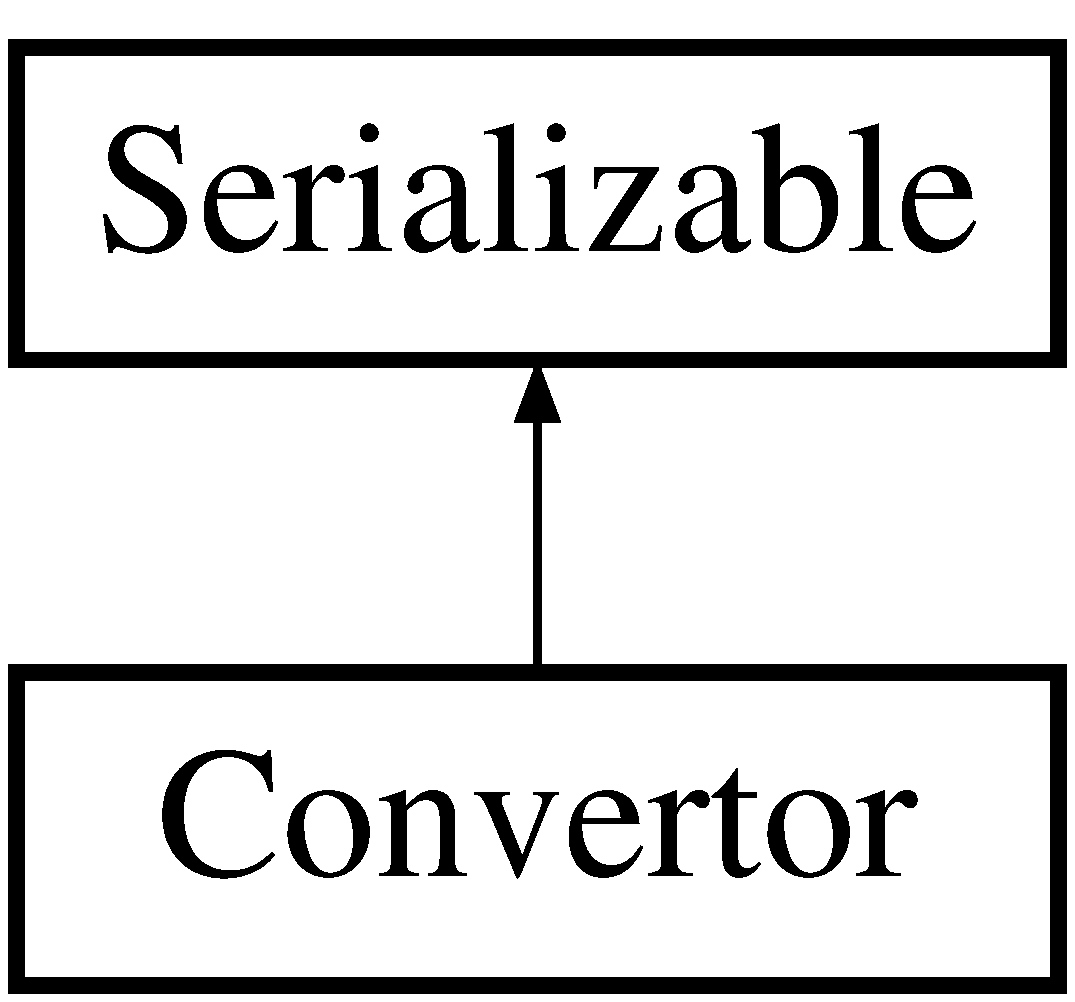
\includegraphics[height=2.000000cm]{classConvertor}
\end{center}
\end{figure}
\subsection*{Public Member Functions}
\begin{DoxyCompactItemize}
\item 
\hypertarget{classConvertor_a2dea9796d78988fca070649c9cdbfe5b}{float {\bfseries get\-Noise} ()}\label{classConvertor_a2dea9796d78988fca070649c9cdbfe5b}

\item 
\hypertarget{classConvertor_a58c496fd28aef5e8f4a583dadf8fce69}{float {\bfseries get\-Line} ()}\label{classConvertor_a58c496fd28aef5e8f4a583dadf8fce69}

\item 
\hypertarget{classConvertor_aab6705c174e40a52fe89c7838ec54127}{float {\bfseries get\-Distortion} ()}\label{classConvertor_aab6705c174e40a52fe89c7838ec54127}

\item 
\hypertarget{classConvertor_a43320d5151ecb614c9af287565186b49}{float {\bfseries get\-D\-N\-R} ()}\label{classConvertor_a43320d5151ecb614c9af287565186b49}

\item 
\hypertarget{classConvertor_aad9a1d5cf8d6385931ae2ab23121d8fc}{float {\bfseries get\-Peak\-Amp} ()}\label{classConvertor_aad9a1d5cf8d6385931ae2ab23121d8fc}

\item 
\hypertarget{classConvertor_ad2102ac186360e51d742209368cf4fdb}{float {\bfseries get\-Min\-Amp} ()}\label{classConvertor_ad2102ac186360e51d742209368cf4fdb}

\item 
\hypertarget{classConvertor_aeea4867b609da0047ecb27e450e79aa8}{void {\bfseries set\-Sample} (\hyperlink{classSample}{Sample} sample)}\label{classConvertor_aeea4867b609da0047ecb27e450e79aa8}

\item 
\hypertarget{classConvertor_ad167bf64d6553655c67d8db98c194391}{\hyperlink{classSample}{Sample} {\bfseries get\-Sample} ()}\label{classConvertor_ad167bf64d6553655c67d8db98c194391}

\item 
\hypertarget{classConvertor_a12a3bf6abbcb8db546d1b0ef3e1b3bf3}{\hyperlink{classSample}{Sample} {\bfseries read\-In\-Sample} ()}\label{classConvertor_a12a3bf6abbcb8db546d1b0ef3e1b3bf3}

\item 
\hypertarget{classConvertor_ad23614472dcf0f3575be36da6989163a}{void {\bfseries read\-Out\-Sample} ()}\label{classConvertor_ad23614472dcf0f3575be36da6989163a}

\end{DoxyCompactItemize}


\subsection{Detailed Description}
\begin{DoxyAuthor}{Author}
Taylor 
\end{DoxyAuthor}


The documentation for this class was generated from the following file\-:\begin{DoxyCompactItemize}
\item 
Convertor.\-java\end{DoxyCompactItemize}

\hypertarget{classNoiseFunction}{\section{Noise\-Function Class Reference}
\label{classNoiseFunction}\index{Noise\-Function@{Noise\-Function}}
}
Inheritance diagram for Noise\-Function\-:\begin{figure}[H]
\begin{center}
\leavevmode
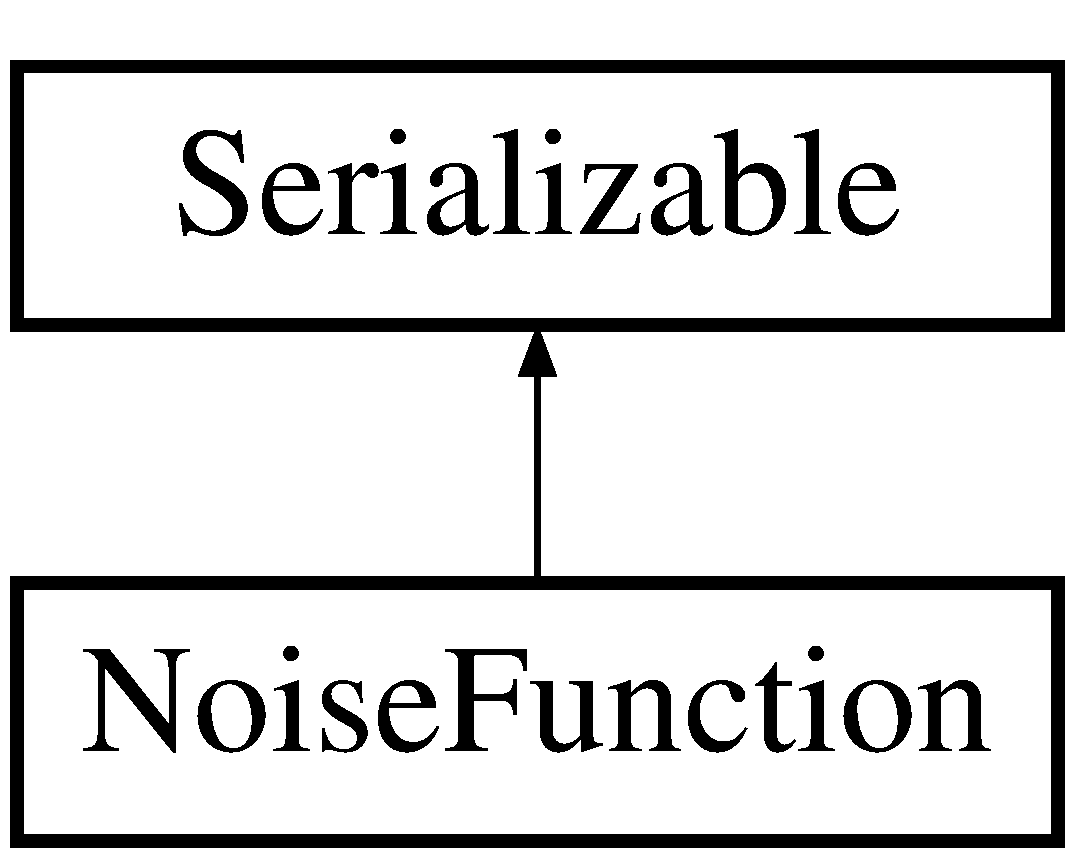
\includegraphics[height=2.000000cm]{classNoiseFunction}
\end{center}
\end{figure}
\subsection*{Public Member Functions}
\begin{DoxyCompactItemize}
\item 
\hyperlink{classSample}{Sample} \hyperlink{classNoiseFunction_a990650302a923a44f1c3504f1724628d}{Add\-Noise} (\hyperlink{classSample}{Sample} sample, float variance, float threshold)
\item 
\hypertarget{classNoiseFunction_a82388ad54f20613f9575d68f07dbc4a2}{\hyperlink{classSample}{Sample} {\bfseries Remove\-Noise} (\hyperlink{classSample}{Sample} sample)}\label{classNoiseFunction_a82388ad54f20613f9575d68f07dbc4a2}

\end{DoxyCompactItemize}


\subsection{Detailed Description}
\begin{DoxyAuthor}{Author}
no\-\_\-author 
\end{DoxyAuthor}


\subsection{Member Function Documentation}
\hypertarget{classNoiseFunction_a990650302a923a44f1c3504f1724628d}{\index{Noise\-Function@{Noise\-Function}!Add\-Noise@{Add\-Noise}}
\index{Add\-Noise@{Add\-Noise}!NoiseFunction@{Noise\-Function}}
\subsubsection[{Add\-Noise}]{\setlength{\rightskip}{0pt plus 5cm}{\bf Sample} Noise\-Function.\-Add\-Noise (
\begin{DoxyParamCaption}
\item[{{\bf Sample}}]{sample, }
\item[{float}]{variance, }
\item[{float}]{threshold}
\end{DoxyParamCaption}
)\hspace{0.3cm}{\ttfamily [inline]}}}\label{classNoiseFunction_a990650302a923a44f1c3504f1724628d}
Add a certain amount of noise to a \hyperlink{classSample}{Sample}. 
\begin{DoxyParams}{Parameters}
{\em sample} & -\/ The \hyperlink{classSample}{Sample} object. \\
\hline
{\em variance} & -\/ Amount of noise added to each amplitude (1.\-0 -\/ 2.\-0). \\
\hline
{\em threshold} & -\/ Maximum amplitude to add noise to (0 -\/ 1.\-0). \\
\hline
\end{DoxyParams}


The documentation for this class was generated from the following file\-:\begin{DoxyCompactItemize}
\item 
Noise\-Function.\-java\end{DoxyCompactItemize}

\hypertarget{classSample}{\section{Sample Class Reference}
\label{classSample}\index{Sample@{Sample}}
}
Inheritance diagram for Sample\-:\begin{figure}[H]
\begin{center}
\leavevmode
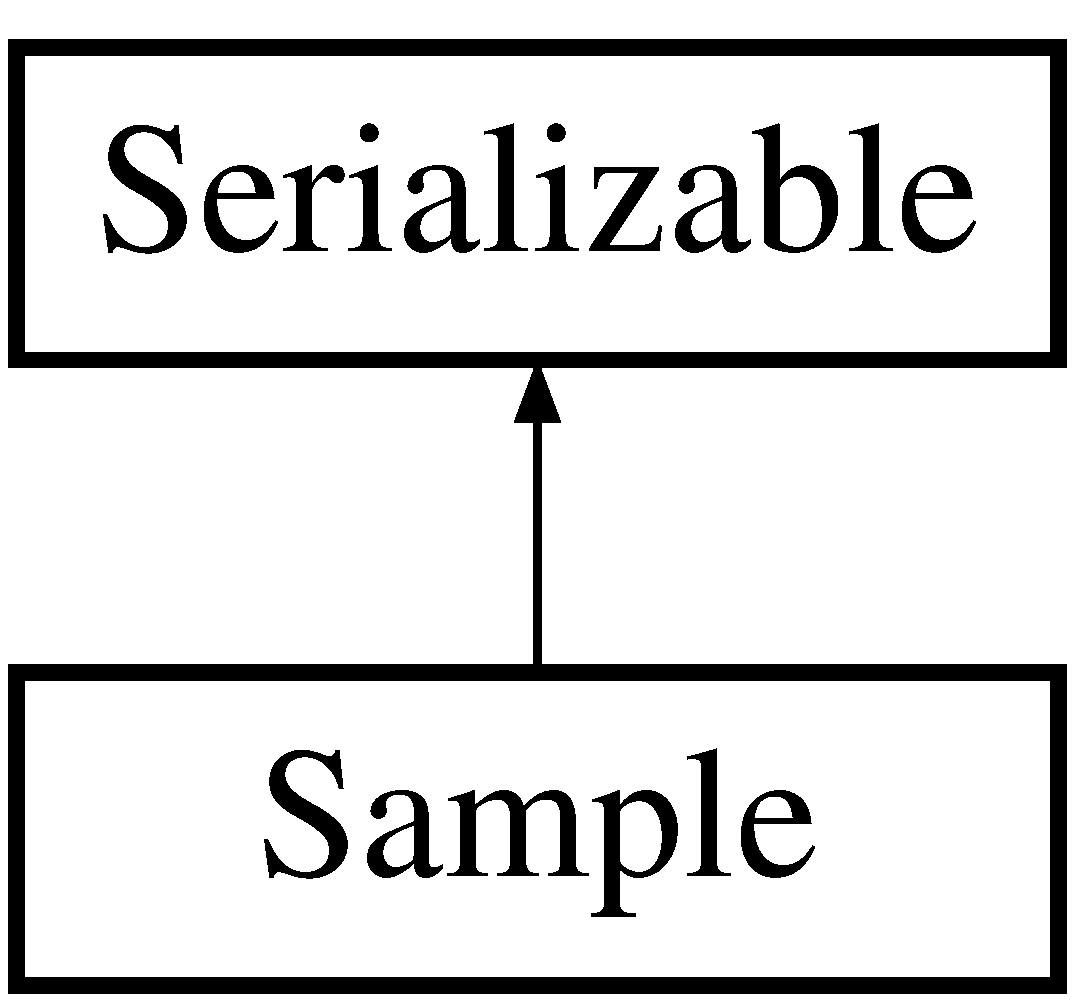
\includegraphics[height=2.000000cm]{classSample}
\end{center}
\end{figure}
\subsection*{Public Member Functions}
\begin{DoxyCompactItemize}
\item 
\hypertarget{classSample_a40304633ec45a48ee9094e0e62e98408}{String {\bfseries get\-File\-Name} ()}\label{classSample_a40304633ec45a48ee9094e0e62e98408}

\item 
\hypertarget{classSample_a90ee5c6a6c77b54ffee2aa4821449a86}{short {\bfseries get\-Format\-Tag} ()}\label{classSample_a90ee5c6a6c77b54ffee2aa4821449a86}

\item 
\hypertarget{classSample_a912e1af0699075fa585f45f422259a47}{short {\bfseries get\-Channels} ()}\label{classSample_a912e1af0699075fa585f45f422259a47}

\item 
\hypertarget{classSample_a2cfd553896e886d141da193e7e8c4242}{int {\bfseries get\-Samples\-Per\-Sec} ()}\label{classSample_a2cfd553896e886d141da193e7e8c4242}

\item 
\hypertarget{classSample_a2dfcf54f79f8ff574483c1596b1e176e}{int {\bfseries get\-Avg\-Bytes\-Per\-Sec} ()}\label{classSample_a2dfcf54f79f8ff574483c1596b1e176e}

\item 
\hypertarget{classSample_a749821370db634f450a6c73855f5be00}{short {\bfseries get\-Block\-Align} ()}\label{classSample_a749821370db634f450a6c73855f5be00}

\item 
\hypertarget{classSample_a4d24818b4d18332c99e49b000fe23db3}{short {\bfseries get\-Bits\-Per\-Sample} ()}\label{classSample_a4d24818b4d18332c99e49b000fe23db3}

\item 
\hypertarget{classSample_a806d1fa05d7cb7600c0c8295652a57ef}{short {\bfseries get\-Ext\-Size} ()}\label{classSample_a806d1fa05d7cb7600c0c8295652a57ef}

\item 
\hypertarget{classSample_a4aba11686c8f5f29259d824d02704f39}{short {\bfseries get\-Valid\-Bits\-Per\-Sample} ()}\label{classSample_a4aba11686c8f5f29259d824d02704f39}

\item 
\hypertarget{classSample_a7c37937011eff8be66dcbdc0706ba1bd}{int {\bfseries get\-Channel\-Mask} ()}\label{classSample_a7c37937011eff8be66dcbdc0706ba1bd}

\item 
\hypertarget{classSample_a8909995784a3ee44df02a8d5b58a4c32}{int {\bfseries get\-Sub\-Format} ()}\label{classSample_a8909995784a3ee44df02a8d5b58a4c32}

\item 
\hypertarget{classSample_af37225c7e2ac53d7e0e34a24e80dba47}{int {\bfseries get\-Sample\-Length} ()}\label{classSample_af37225c7e2ac53d7e0e34a24e80dba47}

\item 
\hypertarget{classSample_a97254a39cf9d058d845b044ed42dc11b}{float\mbox{[}$\,$\mbox{]} {\bfseries get\-Sample\-Data} ()}\label{classSample_a97254a39cf9d058d845b044ed42dc11b}

\item 
\hypertarget{classSample_abe334dfc32a4d11c31af3bee72b2f2c9}{void {\bfseries set\-File\-Name} (String file\-Name)}\label{classSample_abe334dfc32a4d11c31af3bee72b2f2c9}

\item 
\hypertarget{classSample_aee291be6b38d3bd3d73742793af93a6b}{void {\bfseries set\-Format\-Tag} (short format\-Tag)}\label{classSample_aee291be6b38d3bd3d73742793af93a6b}

\item 
\hypertarget{classSample_ac7771244e7a8c2908a6874d804814e60}{void {\bfseries set\-Channels} (short channels)}\label{classSample_ac7771244e7a8c2908a6874d804814e60}

\item 
\hypertarget{classSample_aca851b0629fb100b0a2bf32accfa4802}{void {\bfseries set\-Samples\-Per\-Sec} (int samples\-Per\-Sec)}\label{classSample_aca851b0629fb100b0a2bf32accfa4802}

\item 
\hypertarget{classSample_a0b67b42fb312f5e00c49eb73808f9804}{void {\bfseries set\-Avg\-Bytes\-Per\-Sec} (int avg\-Bytes\-Per\-Sec)}\label{classSample_a0b67b42fb312f5e00c49eb73808f9804}

\item 
\hypertarget{classSample_ab3db7004da9f3273b8e347ba9d259da9}{void {\bfseries set\-Block\-Align} (short block\-Align)}\label{classSample_ab3db7004da9f3273b8e347ba9d259da9}

\item 
\hypertarget{classSample_ab3ddcf6c25fc1816d70a538acbd70a2e}{void {\bfseries set\-Bits\-Per\-Sample} (short bits\-Per\-Sample)}\label{classSample_ab3ddcf6c25fc1816d70a538acbd70a2e}

\item 
\hypertarget{classSample_ae9b83df57a401fb5b06731548c388547}{void {\bfseries set\-Ext\-Size} (short ext\-Size)}\label{classSample_ae9b83df57a401fb5b06731548c388547}

\item 
\hypertarget{classSample_ac6c8c334524662c79fef9aab84699ee5}{void {\bfseries set\-Valid\-Bits\-Per\-Sample} (short valid\-Bits\-Per\-Sample)}\label{classSample_ac6c8c334524662c79fef9aab84699ee5}

\item 
\hypertarget{classSample_a8ffda9f961ce677ccd5247c445bb618b}{void {\bfseries set\-Channel\-Mask} (int channel\-Mask)}\label{classSample_a8ffda9f961ce677ccd5247c445bb618b}

\item 
\hypertarget{classSample_a4faae94bf8a8cc9092893d459d882313}{void {\bfseries set\-Sub\-Format} (int sub\-Format)}\label{classSample_a4faae94bf8a8cc9092893d459d882313}

\item 
\hypertarget{classSample_a94023089dcbeba91439ec81185b61144}{void {\bfseries set\-Sample\-Length} (int sample\-Length)}\label{classSample_a94023089dcbeba91439ec81185b61144}

\item 
\hypertarget{classSample_a18b8f2403e466518ed41d44a5d35c5d7}{void {\bfseries set\-Sample\-Data} (float\mbox{[}$\,$\mbox{]} sample\-Data)}\label{classSample_a18b8f2403e466518ed41d44a5d35c5d7}

\item 
\hypertarget{classSample_acbc5afe50eb34f006f9d71f77d2fae4e}{{\bfseries Sample} (String file\-Name)}\label{classSample_acbc5afe50eb34f006f9d71f77d2fae4e}

\end{DoxyCompactItemize}


\subsection{Detailed Description}
\begin{DoxyAuthor}{Author}
Taylor 
\end{DoxyAuthor}


The documentation for this class was generated from the following file\-:\begin{DoxyCompactItemize}
\item 
Sample.\-java\end{DoxyCompactItemize}

\hypertarget{classSampleReader}{\section{Sample\-Reader Class Reference}
\label{classSampleReader}\index{Sample\-Reader@{Sample\-Reader}}
}
Inheritance diagram for Sample\-Reader\-:\begin{figure}[H]
\begin{center}
\leavevmode
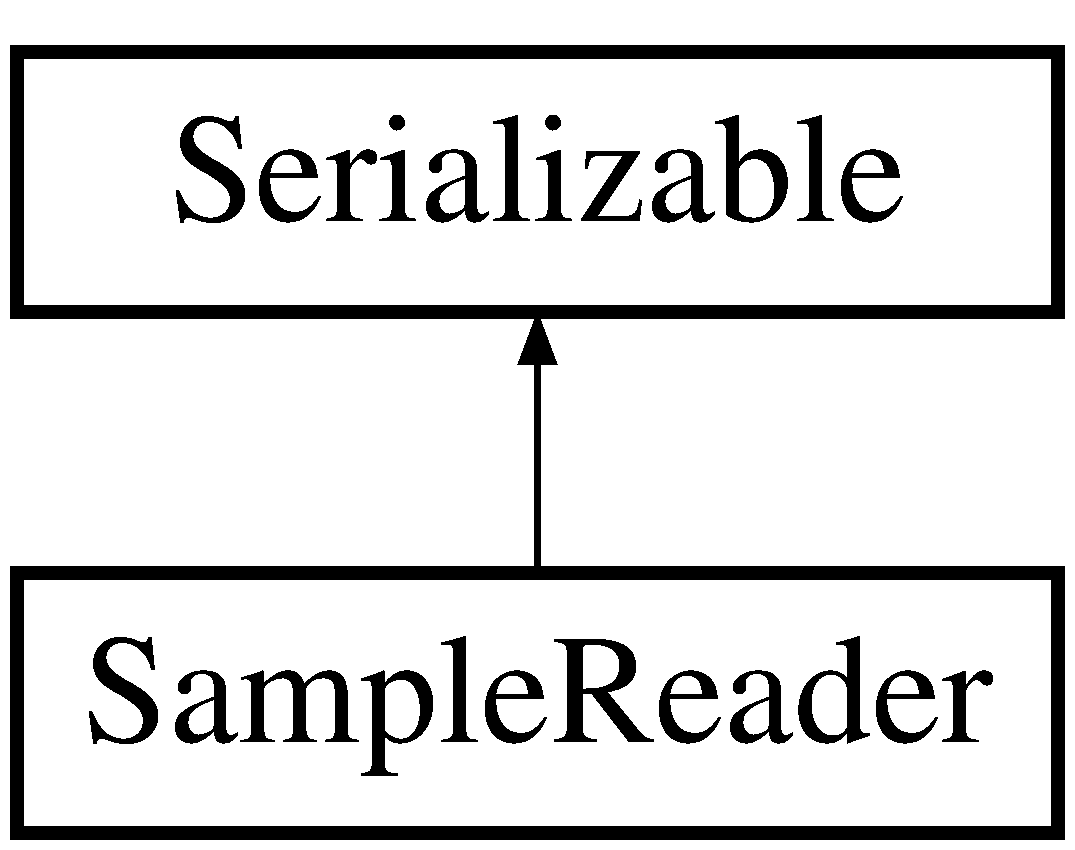
\includegraphics[height=2.000000cm]{classSampleReader}
\end{center}
\end{figure}
\subsection*{Public Member Functions}
\begin{DoxyCompactItemize}
\item 
\hypertarget{classSampleReader_af60a9629ef51bde1f99f61f980fce2c4}{\hyperlink{classSample}{Sample} {\bfseries read\-From\-File} (String file)}\label{classSampleReader_af60a9629ef51bde1f99f61f980fce2c4}

\item 
\hypertarget{classSampleReader_a5c2d1e125397a6d69448ded32878471a}{int {\bfseries read\-Out\-To\-File} (\hyperlink{classSample}{Sample} sample)}\label{classSampleReader_a5c2d1e125397a6d69448ded32878471a}

\end{DoxyCompactItemize}


\subsection{Detailed Description}
\begin{DoxyAuthor}{Author}
Taylor 
\end{DoxyAuthor}


The documentation for this class was generated from the following file\-:\begin{DoxyCompactItemize}
\item 
Sample\-Reader.\-java\end{DoxyCompactItemize}

%--- End generated contents ---

% Index
\newpage
\phantomsection
\addcontentsline{toc}{chapter}{Index}
\printindex

\end{document}
